\documentclass{article}
\usepackage[utf8]{inputenc}

\usepackage{verbatimbox}

\usepackage{graphicx, float, caption, subcaption}
\usepackage{tabularx,booktabs,ragged2e,caption}
\usepackage{makecell}
\newcolumntype{L}{>{\RaggedRight\arraybackslash}X}
\newcolumntype{C}{>{\Centering\arraybackslash}X}


\setlength{\parskip}{1em}
\setlength{\parindent}{0em}

\usepackage{listings}
\usepackage{xcolor}

%CODING SETTINGS
\definecolor{codegreen}{rgb}{0,0.6,0}
\definecolor{codegray}{rgb}{0.5,0.5,0.5}
\definecolor{codepurple}{rgb}{0.58,0,0.82}
\definecolor{backcolour}{rgb}{0.95,0.95,0.92}

\lstdefinestyle{mystyle}{
    backgroundcolor=\color{backcolour},   
    commentstyle=\color{codegreen},
    keywordstyle=\color{magenta},
    numberstyle=\tiny\color{codegray},
    stringstyle=\color{codepurple},
    basicstyle=\ttfamily\footnotesize,
    breakatwhitespace=false,         
    breaklines=true,                 
    captionpos=b,                    
    keepspaces=true,                 
    numbers=left,                    
    numbersep=5pt,                  
    showspaces=false,                
    showstringspaces=false,
    showtabs=false,                  
    tabsize=2
}

\lstset{style=mystyle}

\title{ECS231 Final Project}
\author{Yu-Cheng Hwang \\ 918954206}
\date{June 2022}

\begin{document}
\maketitle
\section{Introduction}
\begin{flushleft}
This project mainly focuses on Arnoldi Algorithm. Arnoldi Algorithm has two ways to find out eigenvalues and eigenvectors. One is Standard Arnoldi, we use arbitrary vector $V$ to calculate Gram-Schmidt for $k$ times to retrieve eigenvalues. The other one is re-orthogonal method. Because there are some errors(or deviation) when we calculate Gram-Schmidt, we need to proceed Gram-Schmidt procedure again to reduce the deviation. Lastly, we want to implement $A-\tau I$ to find out shift and inverse eigenvalues and eigenvectors.
\end{flushleft}
\section{Arnoldi Algorithm without re-orthogonalization}
\subsection{Code}
\begin{lstlisting}[language=Matlab, caption=Arnoldi-without-re-orthogonalization.m]
load west0479
A = west0479;
%k = 20;

% exact eigenvalue
lam = eig(full(A));
figure(1)
hold on
plot(real(lam),imag(lam),'r+');

idx = 1;
%% start calculate range k
for k = 10:10:100
n = length(A);
V = zeros(n,k); % orthonormal basis
H = zeros(k,k); % upper Hessenberg matrix
v = ones(n,1);

V(:,1) = v/norm(v);

% Gram-Schmidt
for j = 1:k
V(:,j+1) = A*V(:,j); % compute w

for i = 1:j
H(i,j) = V(:,i)'*V(:,j+1);
V(:,j+1) = V(:,j+1)-H(i,j)*V(:,i);
end
% normalization
H(j+1,j) = norm(V(:,j+1));

if H(j+1,j) == 0
    break;
else
V(:,j+1) = V(:,j+1)/H(j+1,j);
% compute residual
Ra(j,idx) = norm(A*V(:,j) - V(:,j+1)*H(:,j)');
Rb(j,idx) = norm(speye(k) - V(:,j+1)'*V(:,j+1));
end

end

H(k+1,:) = []; 
Rz = eig(full(H));
plot(real(Rz),imag(Rz),'bo');

% calculate relative errors
lumk = max(lam);
muk = max(Rz);
relerrar(idx,:) = abs(lumk - muk) / abs(lumk);
idx = idx + 1;

%% end of the range k
end
hold off

\end{lstlisting}
\subsection{Results}
\subsubsection{Real Eigenvalues}
\begin{flushleft}
As we can see in the picture, red cross is the original eigenvalues calculated by Matlab, blue circle is the Arnoldi Algorithm's eigenvalues.

Arnodi Algorithm first calculate the eigenvalue from the outside, then converge into inner circle as we see in the figure.
\end{flushleft}
\begin{figure}[H]
    \centering
    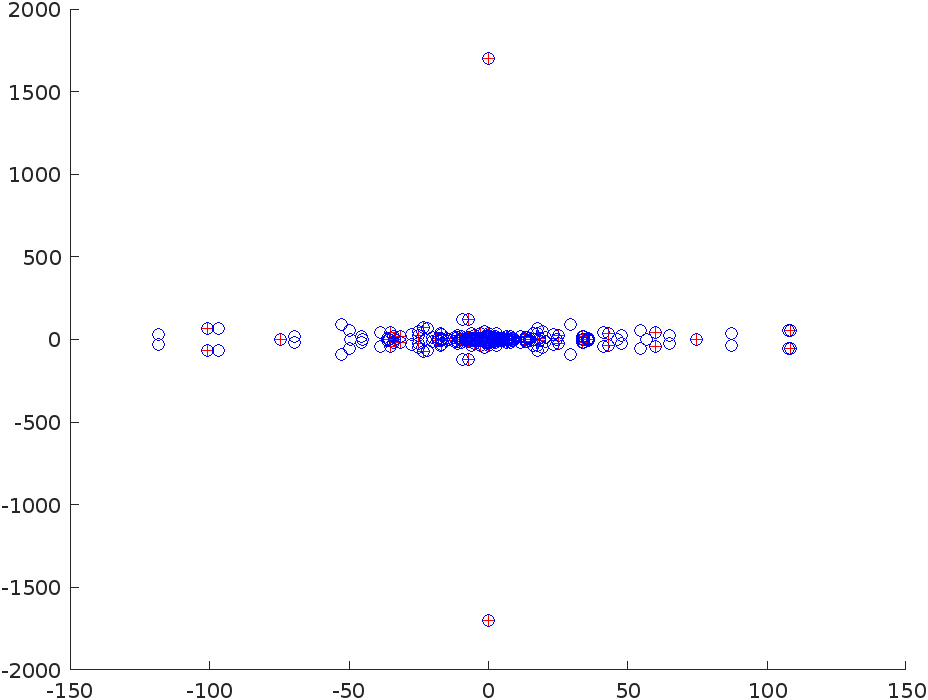
\includegraphics[width=1\textwidth]{arnoldi1.png}
    \caption{Real Eigenvalues and Arnoldi}
    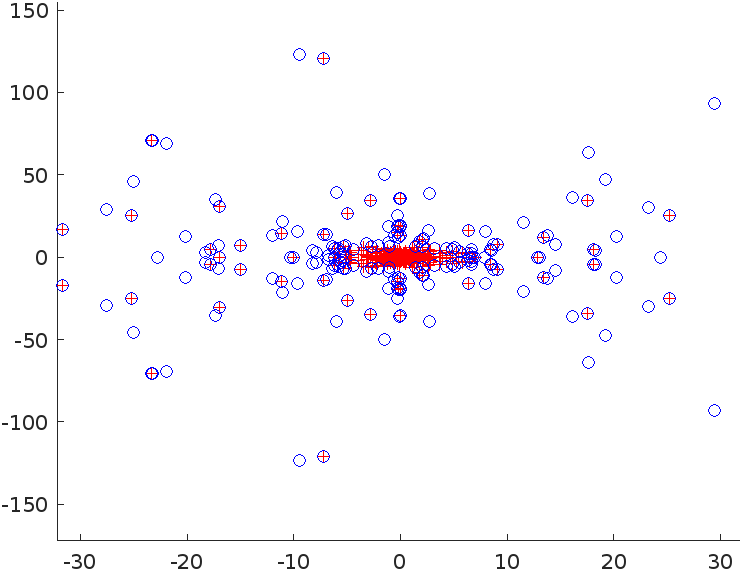
\includegraphics[width=1\textwidth]{arnoldi4.png}
    \caption{Closer Look}
    \label{fig:arnoldi}
\end{figure}
\subsubsection{Residual}
\begin{itemize}
    \item $||AV_j-V_{j+1}\hat{H_j}||$\\
    \\
    When $j$ increases from like $10$ to $20$, it will increase from  $1.5216e^3$ to $5.3781e^3$, however, when we increase $j$ to like $30$, $40$...till $100$, the residual will become smaller to $e^5$, for example, when $j=100$, the value will be $3.1201e^5$.
    \item $||I-J^H_{j+1}V_{j+1}||$\\
    \\
    For $j=10,20,30...100$, the residual value will be $9,19,29...99$.
\end{itemize}
\section{Arnoldi Algorithm with re-orthogonalization}
\subsection{Code}
\begin{lstlisting}[language=Matlab, caption=Arnoldi-with-re-orthogonalization.m]
load west0479
A = west0479;
%k = 20;

% exact eigenvalue
lam = eig(full(A));
figure(2)
hold on
plot(real(lam),imag(lam),'r+');

idx = 1;
%% start calculate range k
for k = 10:10:100
n = length(A);
V = zeros(n,k); % orthonormal basis
H = zeros(k,k); % upper hessenberg matrix
v = ones(n,1);

V(:,1) = v/norm(v);

% Gram-Schmidt
for j = 1:k
V(:,j+1) = A*V(:,j); % compute w

for i = 1:j
H(i,j) = V(:,i)'*V(:,j+1);
V(:,j+1) = V(:,j+1)-H(i,j)*V(:,i);
end
% normalization
H(j+1,j) = norm(V(:,j+1));

% -->reorthogonalization process HERE?
% without any if statement
for l = 1:j
mu = V(:,l)'*V(:,j+1);
V(:,j+1) = V(:,j+1)-V(:,l)*mu;
H(l,j) = H(l,j) + mu;
end
H(j+1, j) = norm(V(:,j+1));

V(:,j+1) = V(:,j+1)/H(j+1,j);
% compute residual
Ra(j,idx) = norm(A*V(:,j) - V(:,j+1)*H(:,j)');
Rb(j,idx) = norm(speye(k) - V(:,j+1)'*V(:,j+1));
end

H(k+1,:) = []; 
Rz = eig(full(H));
plot(real(Rz),imag(Rz),'bo');

% calculate relative errors
lumk = max(lam);
muk = max(Rz);
relerror(idx,:) = abs(lumk - muk) / abs(lumk);
idx = idx + 1;
%% end of the range k
end
hold off
\end{lstlisting}
\subsection{Results}
\subsubsection{Real Eigenvalues and Arnoldi Reorthogonalization Algorithms}
\begin{flushleft}
As we can see in the figure 2, the result is very close to Arnoldi without orthogonalization, but we will inspect the relative error to see the differences between both of them.
\end{flushleft}
\begin{figure}[H]
    \centering
    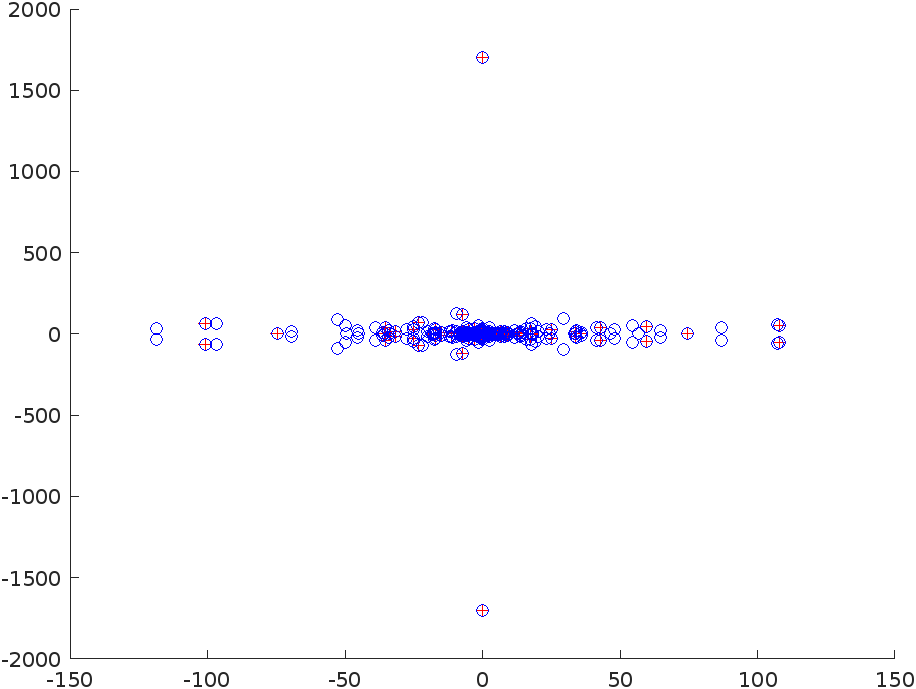
\includegraphics[width=1\textwidth]{arnoldi2.png}
    \caption{Real Eigenvalues and Arnoldi Reorthogonalization}
    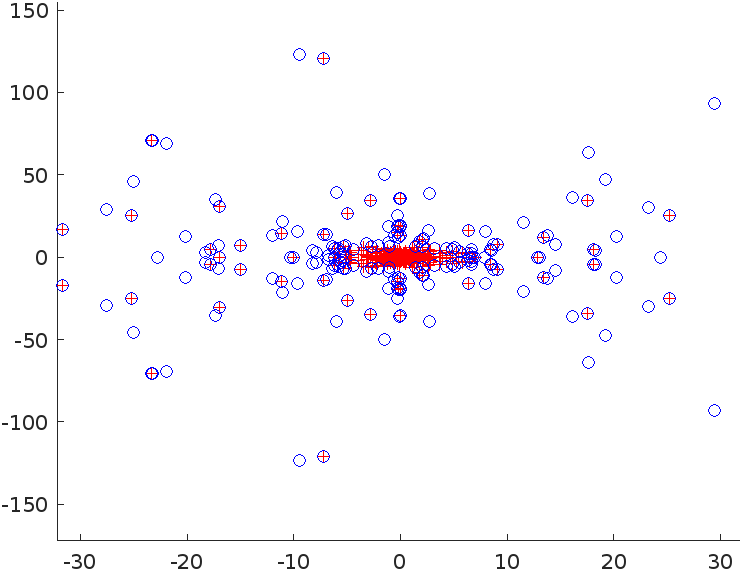
\includegraphics[width=1\textwidth]{arnoldi4.png}
    \caption{Closer Look}
    \label{fig:arnoldi}
\end{figure}
\subsubsection{Residual}
\begin{itemize}
    \item $||AV_j-V_{j+1}\hat{H_j}||$\\
    \\
    We can find out that residual results are similar to Standard Arnoldi(without orthogonalization).When $j$ increases from like $10$ to $20$, it will increase from  $1.5216e^3$ to $5.3781e^3$, however, when we increase $j$ to like $30$, $40$...till $100$, the residual will become smaller to $e^5$, for example, when $j=100$, the value will be $3.1201e^5$.
    \item $||I-J^H_{j+1}V_{j+1}||$\\
    \\
    For $j=10,20,30...100$, the residual value will be $9,19,29...99$.
\end{itemize}
\section{Differences between Standard and re-Orthogonalization}
\subsection{Relative Errors}
\begin{flushleft}
We can use relative errors to compare differences between Standard Arnoldi and re-orthogonalization.
\[\frac{|\lambda_k-\mu^{(j)}_k|}{|\lambda_k|}\ for\ k=1,2,3...\]
\end{flushleft}
\begin{figure}[H]
\centering
\begin{minipage}{.5\textwidth}
  \centering
  \includegraphics[width=.4\linewidth]{final/relerrst.png}
  \captionof{figure}{Standard Arnoldi}
  \label{fig:relerr-st}
\end{minipage}%
\begin{minipage}{.5\textwidth}
  \centering
  \includegraphics[width=.4\linewidth]{final/relerror.png}
  \captionof{figure}{re-Orthogonalization Arnoldi}
  \label{fig:relerr-or}
\end{minipage}
\caption*{Relative Errors}
\label{fig:relerr}
\end{figure}
\begin{flushleft}
As we can see, for Standard Arnoldi, the relative error will decrease from $e^{-10}$ to $e^{-16}$ when we increase our times of loop k from $10$ to $100$. On the other hand, with re-orthogonalization, the relative error will decrease more than Standard Arnoldi.
\end{flushleft}
\subsection{Relative Errors Figures}
\begin{figure}[H]
    \centering
    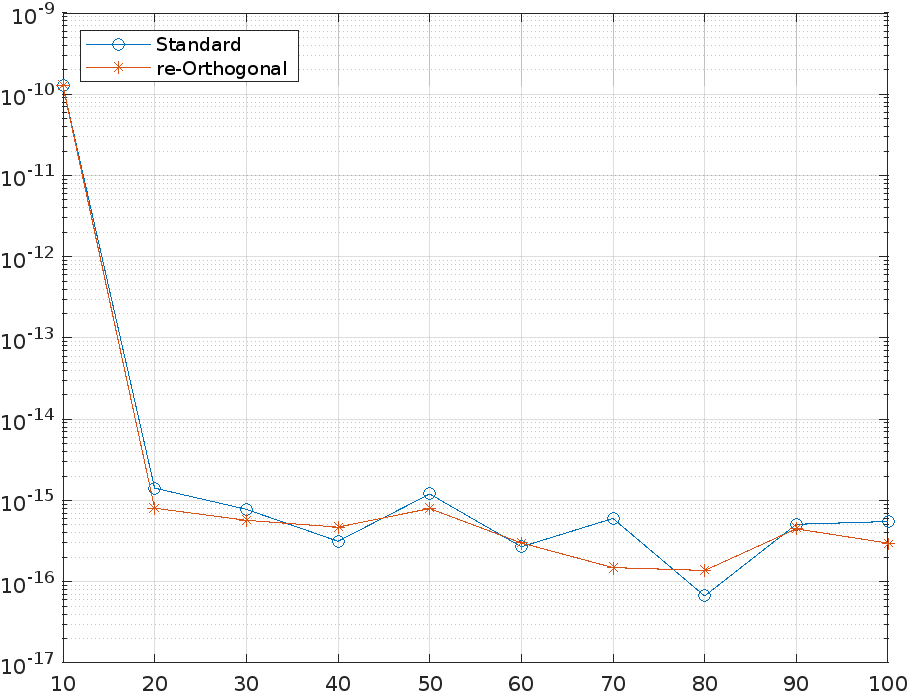
\includegraphics[width=1\textwidth]{relerr_compare.png}
    \caption{Comparing between Standard and re-Orthogonal Arnoldi}
    \label{fig:relerr}
\end{figure}
\section{Two Large Test Metrices}
\subsection{HB/1138\_bus}
\begin{flushleft}
\begin{itemize}
    \item Usage: Power Network Problem
    \item Describe: The optimal power flow problem is concerned with finding and optimal operating point of a power system, which minimized a certain objective function (e.g. power loss or generation cost) subject to network and physical constraints.
    \item Size: $1138*1138$
    \item None zeros: $4054$
\end{itemize}
\end{flushleft}
\subsubsection{Code}
\begin{lstlisting}[language=Matlab, caption=hb1138.m]
in = load('1138bus.mat');
A = in.Problem.A;

idx = 1;
%% start calculate range k
for k = 10:10:100
n = length(A);
V = zeros(n,k); % orthonormal basis
H = zeros(k,k); % upper hessenberg matrix
v = ones(n,1);

V(:,1) = v/norm(v);

% Gram-Schmidt
for j = 1:k
V(:,j+1) = A*V(:,j); % compute w

for i = 1:j
H(i,j) = V(:,i)'*V(:,j+1);
V(:,j+1) = V(:,j+1)-H(i,j)*V(:,i);
end
% normalization
%H(j+1,j) = norm(V(:,j+1));

% -->reorthogonalization process HERE?
% without any if statement
for l = 1:j
mu = V(:,l)'*V(:,j+1);
V(:,j+1) = V(:,j+1)-V(:,l)*mu;
H(l,j) = H(l,j) + mu;
end
H(j+1, j) = norm(V(:,j+1));

V(:,j+1) = V(:,j+1)/H(j+1,j);
% compute residual
Ra(j,idx) = norm(A*V(:,j) - V(:,j+1)*H(:,j)');
Rb(j,idx) = norm(ones(k,k) - V(:,j+1)'*V(:,j+1));
end

H(k+1,:) = [];
V(:, k+1) = [];
Rz = eig(full(H));

% calculate relative errors
muk = max(Rz);
RzV = V*Rz;
nomi = norm(A*RzV - muk*RzV);
deno = (norm(full(A)) + abs(muk)) * norm(RzV);
relerrt6(idx,:) = nomi / deno;
idx = idx + 1;
%% end of the range k
end
\end{lstlisting}
\subsubsection{Results}
\subsubsubsection{Relative Errors}
\begin{flushleft}
Because we can not calculate the relative errors with:
\[\frac{|\lambda_k-\mu^{(j)}_k|}{|\lambda_k|}\ for\ k=1,2,3...\]
We need to replace relative errors with relative residual norms:
\[\frac{||A\hat{u}^{(j)}_k-u^{j}_k\hat{u}^{(j)}_k||}{(||A||+|u^{j}_k|)||\hat{u}^{(j)}_k||}\]
We need to calculate Ritz values and Ritz vectors.\\
Figure \ref{fig:task61} shows the relative errors.\\
And \ref{fig:task61fig} shows its residual error figure.
\end{flushleft}
\begin{figure}[H]
    \centering
    \begin{subfigure}{0.5\textwidth}
        \centering
        \includegraphics[width=0.3\textwidth]{task61.png}
        \caption{Relative Errors for HB/1138\_bus}
        \label{fig:task61}
    \end{subfigure}
    \begin{subfigure}{0.5\textwidth}
        \centering
        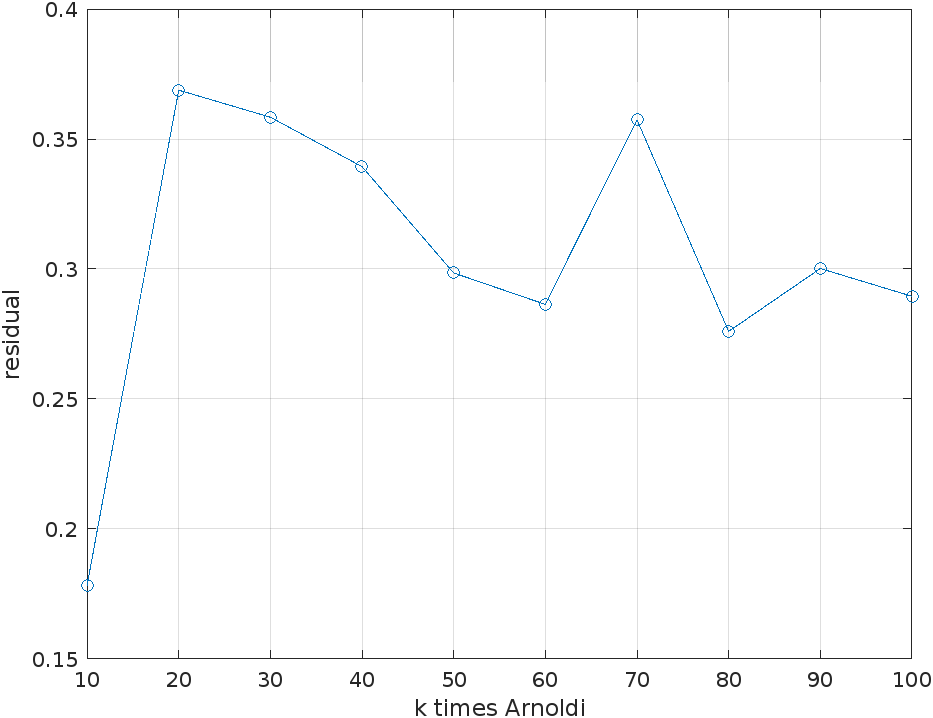
\includegraphics[width=1\textwidth]{task61fig.png}
        \caption{Relative Errors Figure for HB/1138\_bus}
        \label{fig:task61fig}
    \end{subfigure}
    \caption{HB/1138\_bus}
    \label{fig:task61}
\end{figure}
\subsection{GD06\_Java}
\begin{flushleft}
\begin{itemize}
    \item Usage: Directed Graph Problem
    \item Describe: Find out network flows and calculate each node and link's distance, weight, and wastes.
    \item Size: $1538*1538$
    \item None zeros: $8032$
\end{itemize}
\end{flushleft}
\subsubsection{Code}
\begin{lstlisting}[language=Matlab, caption=gd06java.m]
in = load('1138bus.mat/GD06Java.mat'); %input 1138but or GD60Java .mat file
A = in.Problem.A;

idx = 1;
%% start calculate range k
for k = 10:10:100
n = length(A);
V = zeros(n,k); % orthonormal basis
H = zeros(k,k); % upper hessenberg matrix
v = ones(n,1);

V(:,1) = v/norm(v);

% Gram-Schmidt
for j = 1:k
V(:,j+1) = A*V(:,j); % compute w

for i = 1:j
H(i,j) = V(:,i)'*V(:,j+1);
V(:,j+1) = V(:,j+1)-H(i,j)*V(:,i);
end
% normalization
%H(j+1,j) = norm(V(:,j+1));

% -->reorthogonalization process HERE?
% without any if statement
for l = 1:j
mu = V(:,l)'*V(:,j+1);
V(:,j+1) = V(:,j+1)-V(:,l)*mu;
H(l,j) = H(l,j) + mu;
end
H(j+1, j) = norm(V(:,j+1));

V(:,j+1) = V(:,j+1)/H(j+1,j);
% compute residual
Ra(j,idx) = norm(A*V(:,j) - V(:,j+1)*H(:,j)');
Rb(j,idx) = norm(ones(k,k) - V(:,j+1)'*V(:,j+1));
end

H(k+1,:) = [];
V(:, k+1) = [];
Rz = eig(full(H));

% calculate relative errors
muk = max(Rz);
RzV = V*Rz;
nomi = norm(A*RzV - muk*RzV);
deno = (norm(full(A)) + abs(muk)) * norm(RzV);
relerrt6(idx,:) = nomi / deno;
idx = idx + 1;
%% end of the range k
end
\end{lstlisting}
\subsubsection{Results}
\begin{flushleft}
Figure \ref{fig:task62} shows the relative errors.\\
And \ref{fig:task62fig} shows its residual error figure.
\end{flushleft}
\begin{figure}[H]
    \centering
    \begin{subfigure}{0.5\textwidth}
        \centering
        \includegraphics[width=0.3\textwidth]{task62.png}
        \caption{Relative Errors for GD06\_Java}
        \label{fig:task62}
    \end{subfigure}
    \begin{subfigure}{0.5\textwidth}
        \centering
        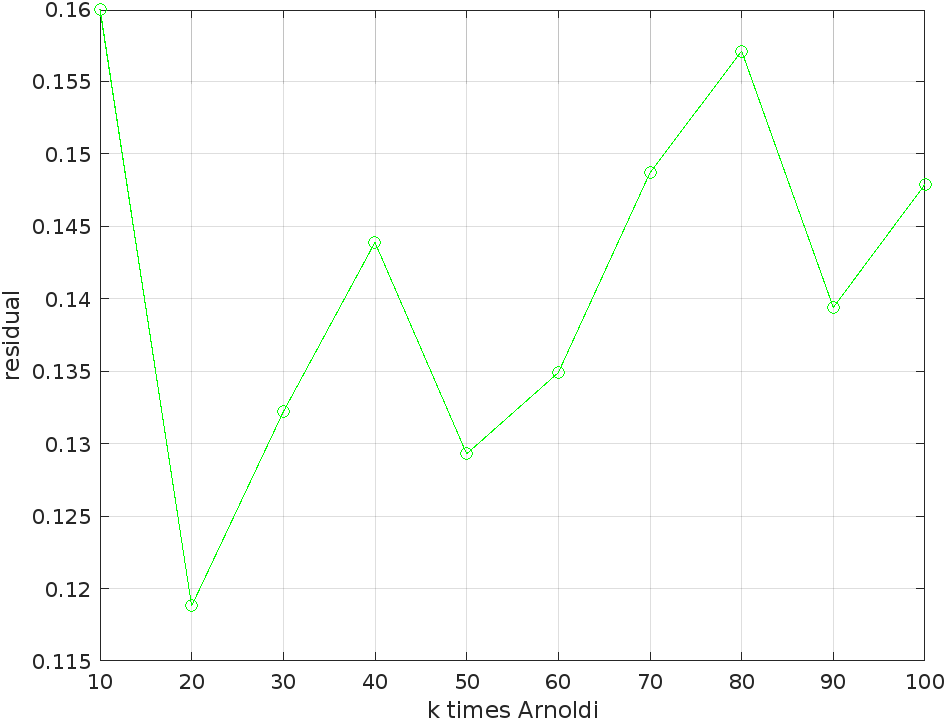
\includegraphics[width=1\textwidth]{task62fig.png}
        \caption{Relative Errors Figure for GD06\_Java}
        \label{fig:task62fig}
    \end{subfigure}
    \caption{GD06\_Java}
    \label{fig:task62}
\end{figure}
\section{Shift and invert the Eigenvalues}
\begin{flushleft}
We are not calculating the original matrix $A$. Instead, we want to calculate the matrix after shifting and inversing.

\[(A-\tau I)^{-1}x = (\lambda-\tau I)^{-1}x\]
Here, we will set $\tau$ to $10, -10, 5$.
\end{flushleft}
\subsection{Code}
\begin{lstlisting}[language=Matlab, caption=shiftandinverse.m]
load west0479
A = west0479;
n = length(A);
%k = 50;

% shift
tau = 10;
A = (A - tau * speye(n));
[L,U,P] = lu(A);
A = inv(U) * inv(L) * inv(P');
%y = L\(P*b);
%x = U\y;

lam = eig(full(A));
figure(5)
hold on
plot(real(lam),imag(lam),'r+');

idx = 1;
%% k
for k = 10:10:50
V = zeros(n,k); % orthonormal basis
H = zeros(k,k); % upper hessenberg matrix
v = ones(n,1);

V(:,1) = v/norm(v);

% Gram-Schmidt
for j = 1:k
V(:,j+1) = A*V(:,j); % compute w

for i = 1:j
H(i,j) = V(:,i)'*V(:,j+1);
V(:,j+1) = V(:,j+1)-H(i,j)*V(:,i);
end
% normalization
H(j+1,j) = norm(V(:,j+1));

% -->reorthogonalization process HERE?
% without any if statement
for l = 1:j
mu = V(:,l)'*V(:,j+1);
V(:,j+1) = V(:,j+1)-V(:,l)*mu;
H(l,j) = H(l,j) + mu;
end
H(j+1, j) = norm(V(:,j+1));

V(:,j+1) = V(:,j+1)/H(j+1,j);
% compute residual
Ra(:,j) = norm(A*V(:,j) - V(:,j+1)*H(:,j)');
Rb(:,j) = norm(speye(k) - V(:,j+1)'*V(:,j+1));
end

H(k+1,:) = []; 
Rz = eig(full(H));
% relative error
lumk = max(lam);
muk = max(Rz);
relerror(idx,:) = abs(lumk - muk) / abs(lumk);
idx = idx + 1;

%% end k
end

Rz = eig(full(H));
plot(real(Rz),imag(Rz),'bo');
hold off
\end{lstlisting}
\subsection{$\tau = 10$}
\begin{flushleft}
In figure \ref{fig:task71}, we can find out that for larger $k$, we will have $0$ relative errors.
\end{flushleft}
\begin{figure}[H]
    \centering
    \begin{subfigure}{0.8\textwidth}
        \centering
        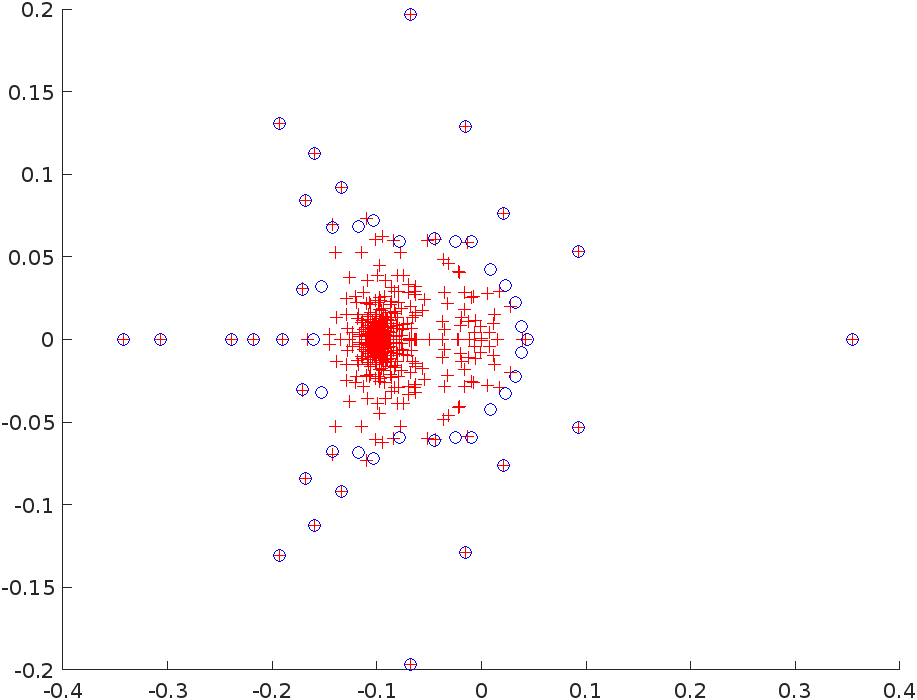
\includegraphics[width=1\textwidth]{task71.png}
        \caption{Eigenvalues and Arnoldi Algorithm}
        \label{fig:task71e}
    \end{subfigure}
    \begin{subfigure}{0.5\textwidth}
        \centering
        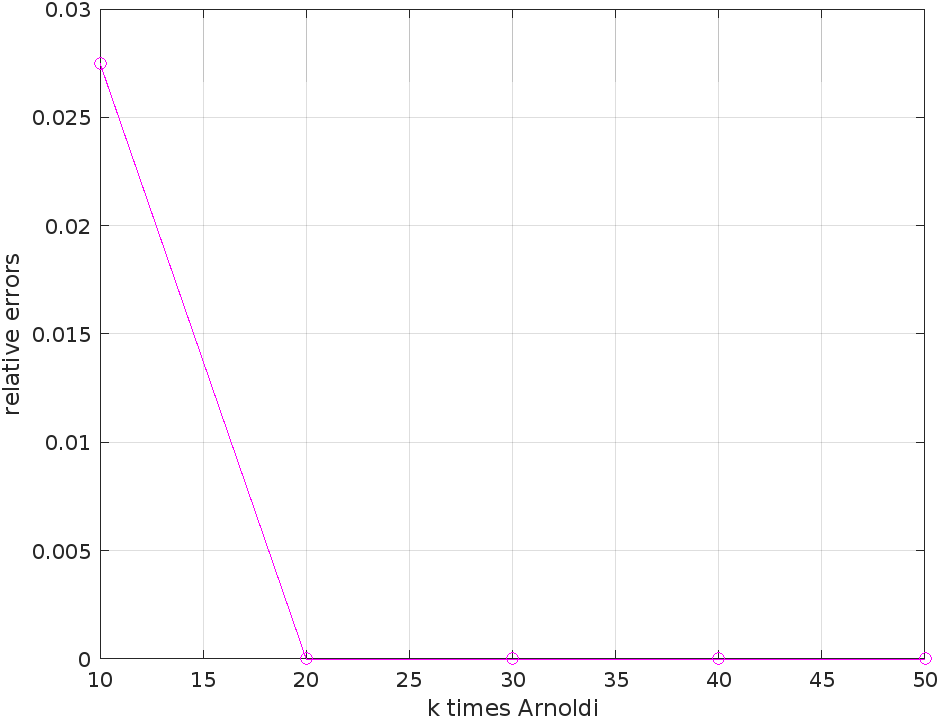
\includegraphics[width=1\textwidth]{final/task71relerr.png}
        \caption{Relative Errors}
        \label{fig:task71relerr}
    \end{subfigure}
    \caption{$\tau=10$}
    \label{fig:task71}
\end{figure}
\subsection{$\tau = 5$}
\begin{flushleft}
In figure \ref{fig:task72}, we can find out that for larger $k$, we will have relative errors close to $0$.
\end{flushleft}
\begin{figure}[H]
    \centering
    \begin{subfigure}{0.8\textwidth}
        \centering
        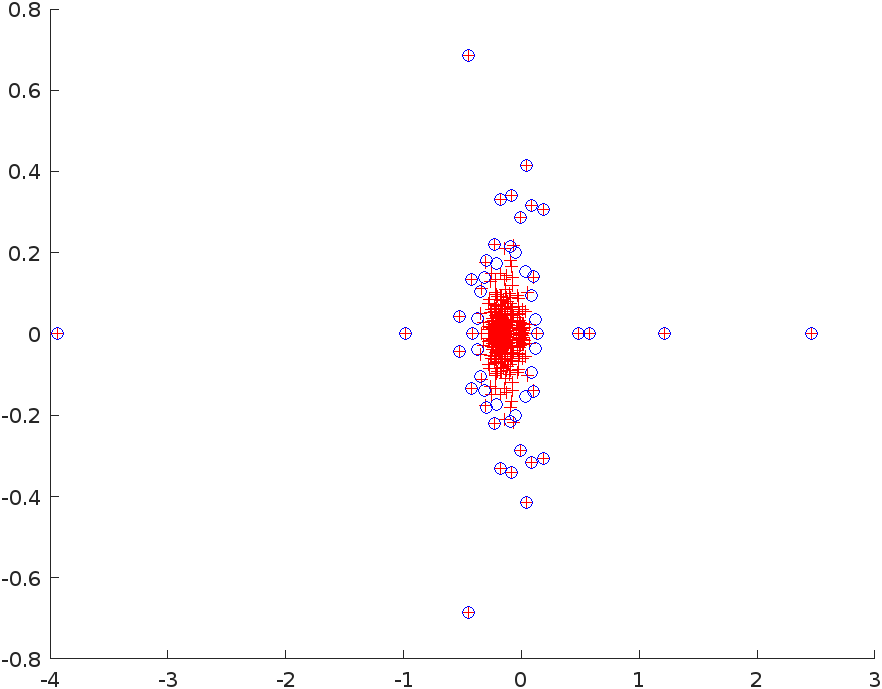
\includegraphics[width=1\textwidth]{task72.png}
        \caption{Eigenvalues and Arnoldi Algorithm}
        \label{fig:task72e}
    \end{subfigure}
    \begin{subfigure}{0.5\textwidth}
        \centering
        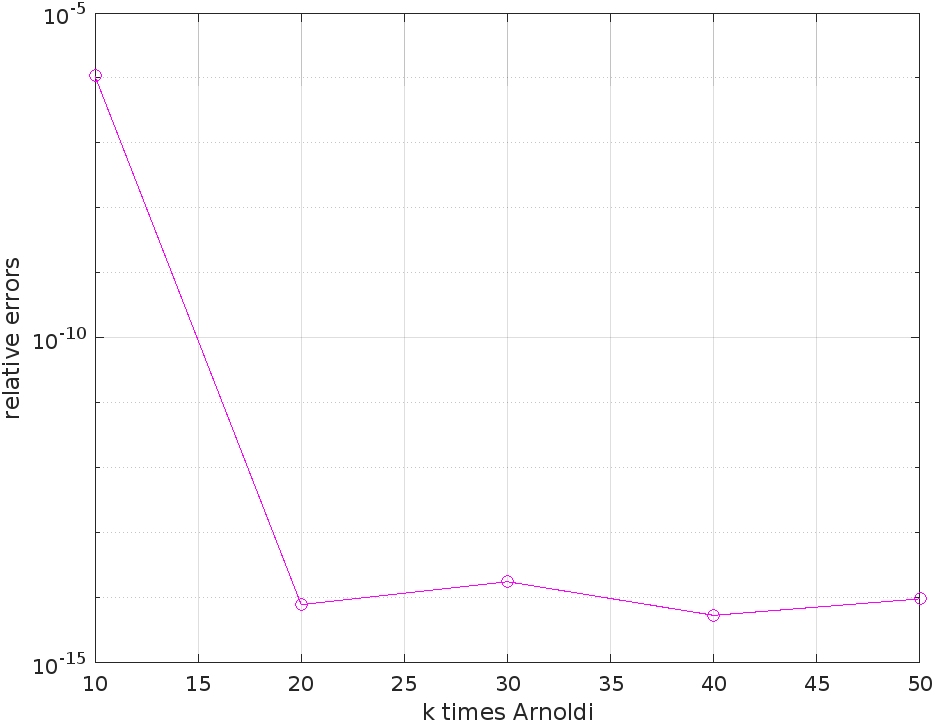
\includegraphics[width=1\textwidth]{final/task72relerr.png}
        \caption{Relative Errors}
        \label{fig:task72relerr}
    \end{subfigure}
    \caption{$\tau=5$}
    \label{fig:task72}
\end{figure}
\subsection{$\tau = -10$}
\begin{flushleft}
In figure \ref{fig:task73}, we can find out that for larger $k$, we will have relative errors close to $0$. And the the most of eigenvalues are near at $X=0$.
\end{flushleft}
\begin{figure}[H]
    \centering
    \begin{subfigure}{0.5\textwidth}
        \centering
        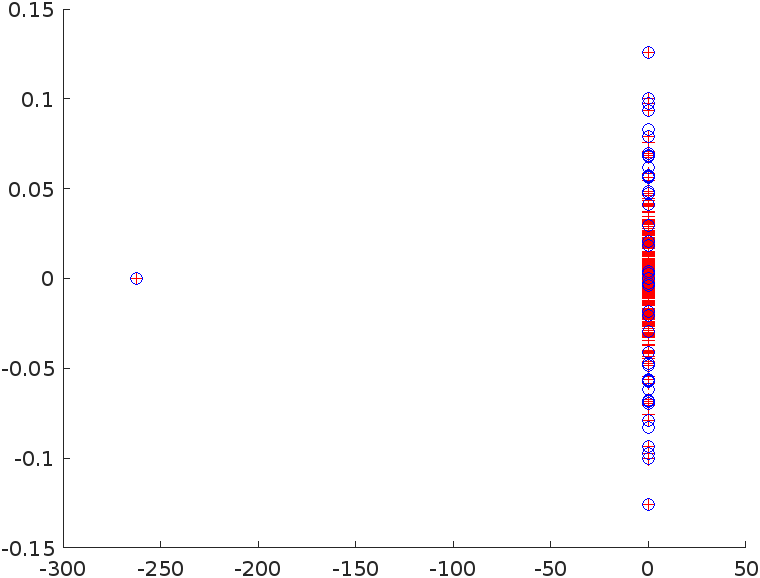
\includegraphics[width=1\textwidth]{task73.png}
        \caption{Eigenvalues and Arnoldi Algorithm}
        \label{fig:task73e}
    \end{subfigure}
    
    \begin{subfigure}{0.5\textwidth}
        \centering
        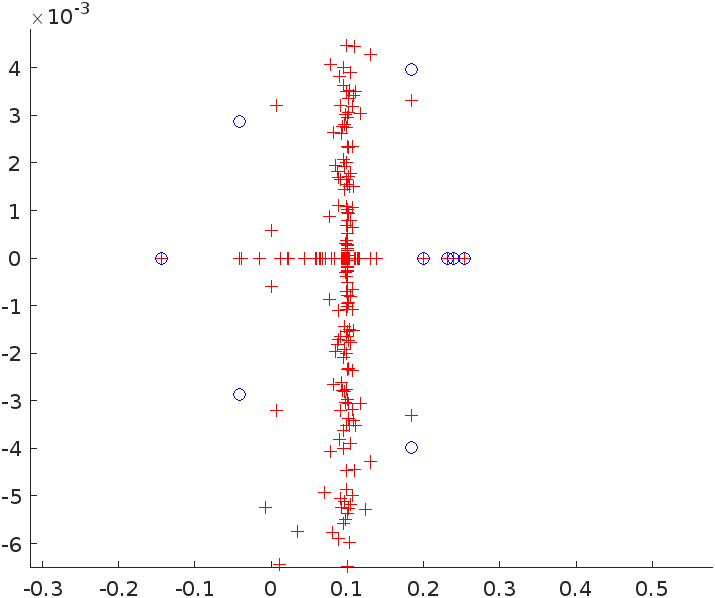
\includegraphics[width=1\textwidth]{task73c.png}
        \caption{Closer look}
        \label{fig:task73ec}
    \end{subfigure}
    
    \begin{subfigure}{0.4\textwidth}
        \centering
        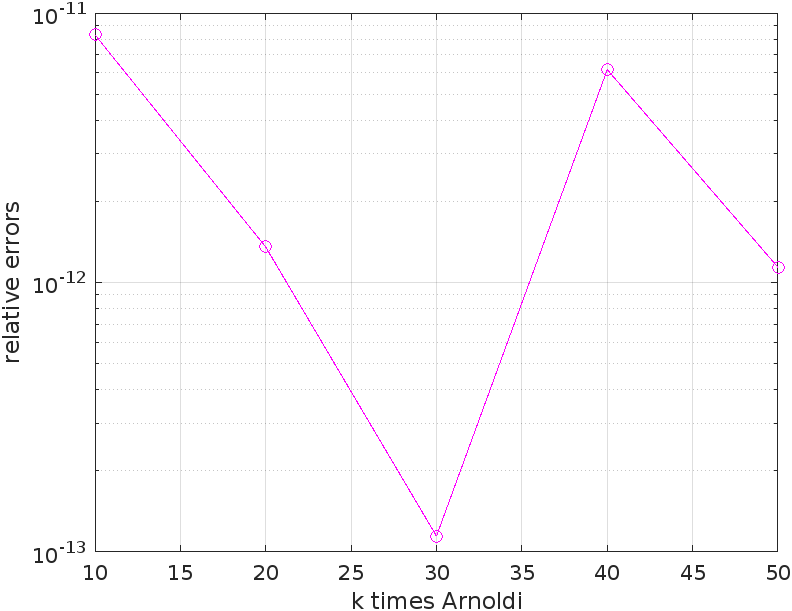
\includegraphics[width=1\textwidth]{final/task73relerr.png}
        \caption{Relative Errors}
        \label{fig:task73relerr}
    \end{subfigure}
    \caption{$\tau=-10$}
    \label{fig:task73}
\end{figure}
\section{Shift and invert the Eigenvalues:Large Matrix}
\subsection{Code}
\begin{lstlisting}[language=Matlab, caption=task8.m]
in = load('1138bus.mat/GD06Java.mat'); %input 1138but or GD60Java .mat file
A = in.Problem.A;
n = length(A);

% shift
tau = -10;
A = (A - tau * speye(n));
[L,U,P] = lu(A);
A = inv(U) * inv(L) * inv(P');

idx = 1;
%% start calculate range k
for k = 10:10:50
V = zeros(n,k); % orthonormal basis
H = zeros(k,k); % upper hessenberg matrix
v = ones(n,1);

V(:,1) = v/norm(v);

% Gram-Schmidt
for j = 1:k
V(:,j+1) = A*V(:,j); % compute w

for i = 1:j
H(i,j) = V(:,i)'*V(:,j+1);
V(:,j+1) = V(:,j+1)-H(i,j)*V(:,i);
end
% normalization
%H(j+1,j) = norm(V(:,j+1));

% -->reorthogonalization process HERE?
% without any if statement
for l = 1:j
mu = V(:,l)'*V(:,j+1);
V(:,j+1) = V(:,j+1)-V(:,l)*mu;
H(l,j) = H(l,j) + mu;
end
H(j+1, j) = norm(V(:,j+1));

V(:,j+1) = V(:,j+1)/H(j+1,j);
% compute residual
Ra(j,idx) = norm(A*V(:,j) - V(:,j+1)*H(:,j)');
Rb(j,idx) = norm(ones(k,k) - V(:,j+1)'*V(:,j+1));
end

H(k+1,:) = [];
V(:, k+1) = [];
Rz = eig(full(H));

% calculate relative errors
muk = max(Rz);
RzV = V*Rz;
nomi = norm(A*RzV - muk*RzV);
deno = (norm(full(A)) + abs(muk)) * norm(RzV);
relerrt6(idx,:) = nomi / deno;
idx = idx + 1;
%% end of the range k
end

figure(81)
X = 10:10:50;
semilogy(X, relerrt6, 'm-o')
xlabel('k times Arnoldi')
ylabel('relative errors')
grid on
\end{lstlisting}
\subsection{Results for HB\_1138}
\subsubsection{$\tau=-10$}
\begin{figure}[H]
    \centering
    \begin{subfigure}{0.4\textwidth}
        \centering
        \includegraphics[width=0.4\textwidth]{task81.png}
        \caption{Convergence}
        \label{fig:task81}
    \end{subfigure}
    \begin{subfigure}{0.6\textwidth}
        \centering
        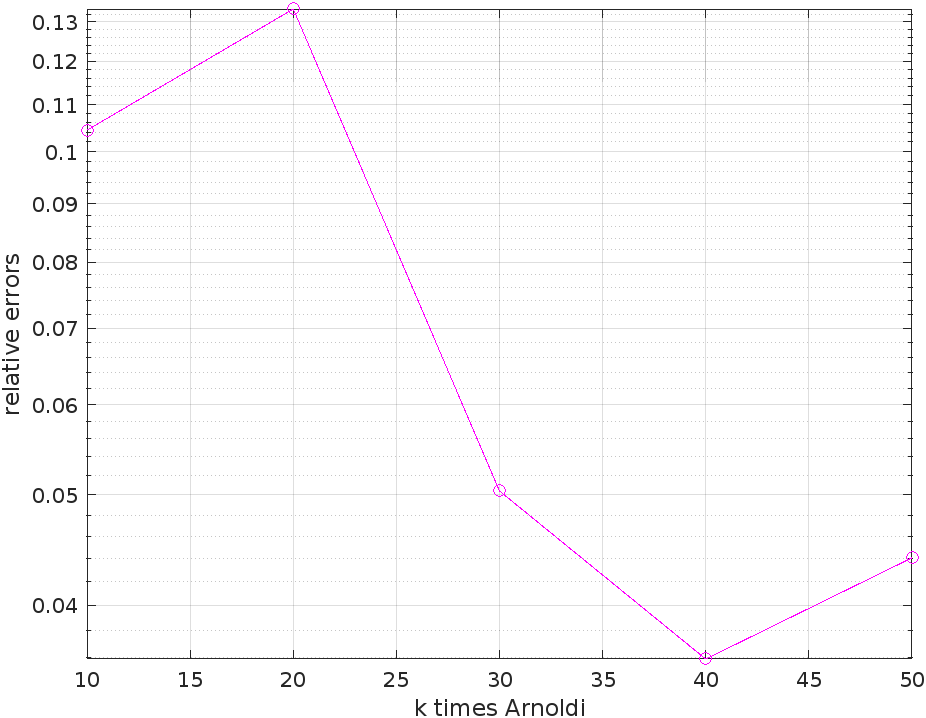
\includegraphics[width=1\textwidth]{task81resi.png}
        \caption{Convergence Figure}
        \label{fig:task81res}
    \end{subfigure}
    \caption{Convergence for HB\_1138}
    \label{fig:task81}
\end{figure}
\subsubsection{$\tau=10$}
\begin{figure}[H]
    \centering
    \begin{subfigure}{0.4\textwidth}
        \centering
        \includegraphics[width=0.4\textwidth]{task811.png}
        \caption{Convergence}
        \label{fig:task811}
    \end{subfigure}
    \begin{subfigure}{0.6\textwidth}
        \centering
        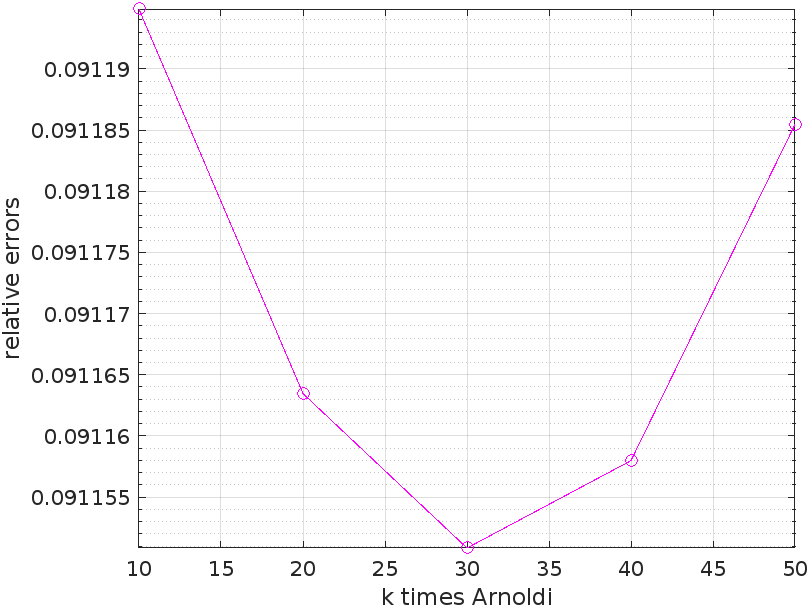
\includegraphics[width=1\textwidth]{task811resi.png}
        \caption{Convergence Figure}
        \label{fig:task811res}
    \end{subfigure}
    \caption{Convergence for HB\_1138}
    \label{fig:task81}
\end{figure}
\subsection{Results for GD06\_JAVA}
\subsubsection{$\tau=-10$}
\begin{figure}[H]
    \centering
    \begin{subfigure}{0.4\textwidth}
        \centering
        \includegraphics[width=0.4\textwidth]{task82.png}
        \caption{Convergence}
        \label{fig:task82}
    \end{subfigure}
    \begin{subfigure}{0.6\textwidth}
        \centering
        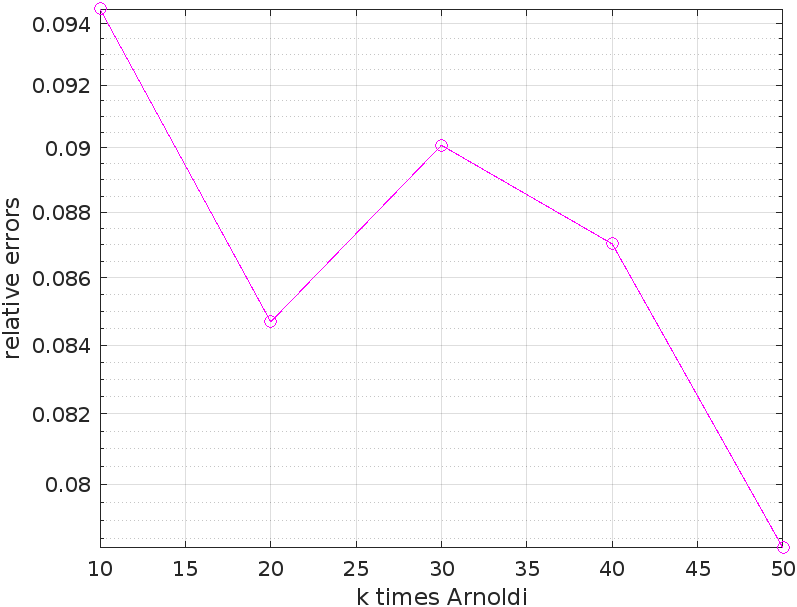
\includegraphics[width=1\textwidth]{task82resi.png}
        \caption{Convergence Figure}
        \label{fig:task82res}
    \end{subfigure}
    \caption{Convergence for GD06\_Java}
    \label{fig:task822}
\end{figure}
\subsubsection{$\tau=10$}
\begin{figure}[H]
    \centering
    \begin{subfigure}{0.4\textwidth}
        \centering
        \includegraphics[width=0.4\textwidth]{task822.png}
        \caption{Convergence}
        \label{fig:task822}
    \end{subfigure}
    \begin{subfigure}{0.6\textwidth}
        \centering
        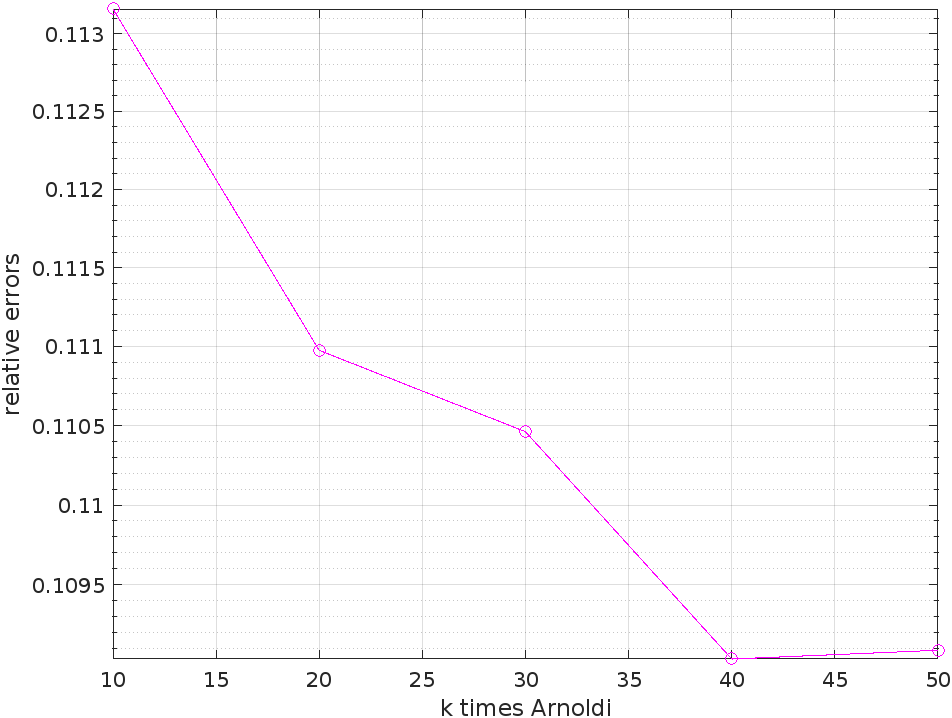
\includegraphics[width=1\textwidth]{task822resi.png}
        \caption{Convergence Figure}
        \label{fig:task822res}
    \end{subfigure}
    \caption{Convergence for GD06\_Java}
    \label{fig:task822}
\end{figure}
\end{document}